U opent het rekeningformulier door in het hoofdmenu op de knop ``Rekeningen'' te klikken. U kunt in dit formulier rekeningen opmaken per pati\"ent of per afdeling. Het formulier bestaat uit een aantal knoppen waarmee U rekeningen kuntbetalen, bekijken en versturen. Hieronder wordt uitlegd hoe dit in zijn werk gaat.\\
\\
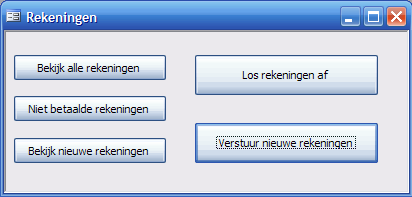
\includegraphics[scale=.8]{rekeningen1}

\section{Rekeningen bekijken} \label{sec: niewe rekeningen}
U kunt de rekeningen bekijken met de knop ``Bekijk alle rekeningen''.
De knop ``Niet betaalde rekeningen'' laat hetzelfde rapport zien, maar
dan alleen met de rekeningen die niet betaald zijn.

\section{Nieuwe rekeningen} \label{sec: nieuwe rekeningen}
Met de knop ``Bekijk nieuwe rekeningen'' kunt U nieuwe rekeningen bekijken en versturen. Door
ze te bekijken opent U een preview met alle nieuwe rekeningen. Door ze te
versturen worden ze opgeslagen in de database en verstuurd op de huidige
datum.

\section{Rekeningen aflossen} \label{sec:rekeningen aflossen}
De knop ``Los rekening af'' opent een venster waarin U een rekening (bij een pati\"ent)
kunt selecteren en vervolgens het uitstaande bedrag (wat al betaald is) kunt
bijwerken met de knop ``Betaal'', nadat U heeft ingevuld hoeveel de patient
betaald heeft.
